\RequirePackage[l2tabu,orthodox]{nag}

% TODO: decide if one-sided/two-sided
%\documentclass[headsepline,footsepline,footinclude=false,fontsize=11pt,paper=a4,listof=totoc,bibliography=totoc,BCOR=12mm,DIV=12]{scrbook} % two-sided
\documentclass[headsepline,footsepline,footinclude=false,oneside,fontsize=11pt,paper=a4,listof=totoc,bibliography=totoc]{scrbook} % one-sided

% TODO: change citation style in settings
\PassOptionsToPackage{table,svgnames,dvipsnames}{xcolor}

\usepackage[utf8]{inputenc}
\usepackage[T1]{fontenc}
\usepackage[sc]{mathpazo}
\usepackage[ngerman,american]{babel}
\usepackage[autostyle]{csquotes}
\usepackage[%
  backend=biber,
  url=false,
  style=numeric,
  maxnames=4,
  minnames=3,
  maxbibnames=99,
  giveninits,
  uniquename=init]{biblatex} % TODO: adapt citation style
\usepackage{graphicx}
\usepackage{scrhack} % necessary for listings package
\usepackage{listings}
\lstdefinestyle{mystyle}{
    basicstyle=\ttfamily\footnotesize,
    breakatwhitespace=false,         
    breaklines=true,                 
    captionpos=b,  
    frame=single,
    keepspaces=true,                 
    numbers=left,                    
    numbersep=5pt,
    numberstyle=\small\color{gray},
    showspaces=false,                
    showstringspaces=false,
    showtabs=false,                  
    tabsize=4
}
\lstset{style=mystyle}
\usepackage{lstautogobble}
\usepackage{tikz}
\usepackage{pgfplots}
\usepackage{pgfplotstable}
\usepackage{booktabs}
\usepackage[final]{microtype}
\usepackage{caption}
\usepackage[hidelinks]{hyperref} % hidelinks removes colored boxes around references and links

\bibliography{bibliography}

\setkomafont{disposition}{\normalfont\bfseries} % use serif font for headings
\linespread{1.05} % adjust line spread for mathpazo font

% Add table of contents to PDF bookmarks
\BeforeTOCHead[toc]{{\cleardoublepage\pdfbookmark[0]{\contentsname}{toc}}}

% Define TUM corporate design colors
% Taken from http://portal.mytum.de/corporatedesign/index_print/vorlagen/index_farben
\definecolor{TUMBlue}{HTML}{0065BD}
\definecolor{TUMSecondaryBlue}{HTML}{005293}
\definecolor{TUMSecondaryBlue2}{HTML}{003359}
\definecolor{TUMBlack}{HTML}{000000}
\definecolor{TUMWhite}{HTML}{FFFFFF}
\definecolor{TUMDarkGray}{HTML}{333333}
\definecolor{TUMGray}{HTML}{808080}
\definecolor{TUMLightGray}{HTML}{CCCCC6}
\definecolor{TUMAccentGray}{HTML}{DAD7CB}
\definecolor{TUMAccentOrange}{HTML}{E37222}
\definecolor{TUMAccentGreen}{HTML}{A2AD00}
\definecolor{TUMAccentLightBlue}{HTML}{98C6EA}
\definecolor{TUMAccentBlue}{HTML}{64A0C8}

% Settings for pgfplots
\pgfplotsset{compat=newest}
\pgfplotsset{
  % For available color names, see http://www.latextemplates.com/svgnames-colors
  cycle list={TUMBlue\\TUMAccentOrange\\TUMAccentGreen\\TUMSecondaryBlue2\\TUMDarkGray\\},
}

% Settings for lstlistings
\lstset{%
  basicstyle=\ttfamily,
  columns=fullflexible,
  autogobble,
  keywordstyle=\bfseries\color{TUMBlue},
  stringstyle=\color{TUMAccentGreen}
}


% TODO: change thesis information
\newcommand*{\getUniversity}{Technische Universität München}
\newcommand*{\getFaculty}{Department of Informatics}
\newcommand*{\getTitle}{A Checkpoint Management System for Embedded Distributed Systems based on the L4 Fiasco.OC and the Genode OS Framework}
\newcommand*{\getTitleGer}{Ein Checkpoint Management System für Eingebettete Verteilte Systeme basierend auf dem L4 Fiasco.OC und dem Genode OS Framework}
\newcommand*{\getAuthor}{Kevin Burton}
\newcommand*{\getDoctype}{Bachelor's Thesis}
\newcommand*{\getSupervisor}{David Werner, M.Sc.}
\newcommand*{\getAdvisor}{Prof. Dr. Claudia Eckert}
\newcommand*{\getSubmissionDate}{15.11.2021}
\newcommand*{\getSubmissionLocation}{Munich}

\begin{document}

% Set page numbering to avoid "destination with the same identifier has been already used" warning for cover page.
% (see https://en.wikibooks.org/wiki/LaTeX/Hyperlinks#Problems_with_Links_and_Pages).
\pagenumbering{alph}
\begin{titlepage}
  % HACK for two-sided documents: ignore binding correction for cover page.
  % Adapted from Markus Kohm's KOMA-Script titlepage=firstiscover handling.
  % See http://mirrors.ctan.org/macros/latex/contrib/koma-script/scrkernel-title.dtx,
  % \maketitle macro.
  \oddsidemargin=\evensidemargin\relax
  \textwidth=\dimexpr\paperwidth-2\evensidemargin-2in\relax
  \hsize=\textwidth\relax

  \centering

  \IfFileExists{logos/tum.pdf}{%
    
\includegraphics[height=20mm]{logos/tum.pdf}
  }{%
    \vspace*{20mm}
  }

  \vspace{5mm}
  {\huge\MakeUppercase{\getFaculty{}}}\\

  \vspace{5mm}
  {\large\MakeUppercase{\getUniversity{}}}\\

  \vspace{20mm}
  {\Large \getDoctype{}}

  \vspace{15mm}
  {\huge\bfseries \getTitle{}}

  \vspace{15mm}
  {\LARGE \getAuthor{}}

  \IfFileExists{logos/faculty.png}{%
    \vfill{}
    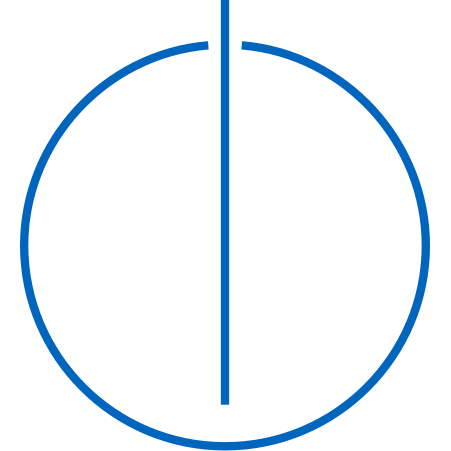
\includegraphics[height=20mm]{logos/faculty.png}
  }{}
\end{titlepage}


\frontmatter{}

\begin{titlepage}
  \centering

  \IfFileExists{logos/tum.pdf}{%
    
\includegraphics[height=20mm]{logos/tum.pdf}
  }{%
    \vspace*{20mm}
  }

  \vspace{5mm}
  {\huge\MakeUppercase{\getFaculty{}}}\\

  \vspace{5mm}
  {\large\MakeUppercase{\getUniversity{}}}\\

  \vspace{20mm}
  {\Large \getDoctype{}}

  \vspace{15mm}
  {\huge\bfseries \getTitle{}}

  \vspace{10mm}
  {\huge\bfseries \foreignlanguage{ngerman}{\getTitleGer{}}}

  \vspace{15mm}
  \begin{tabular}{l l}
    Author:          & \getAuthor{} \\
    Supervisor:      & \getSupervisor{} \\
    Advisor:         & \getAdvisor{} \\
    Submission Date: & \getSubmissionDate{} \\
  \end{tabular}

  \IfFileExists{logos/faculty.png}{%
    \vfill{}
    %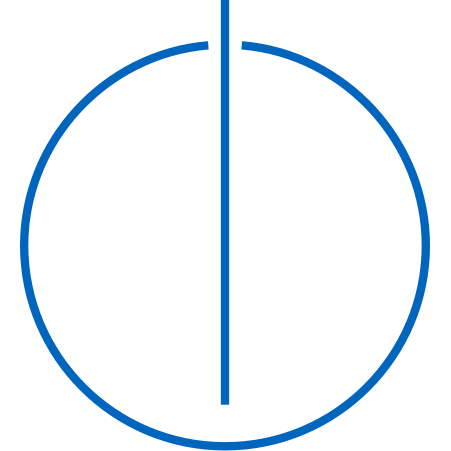
\includegraphics[height=20mm]{logos/faculty.png}
  }{}
\end{titlepage}

\thispagestyle{empty}
\vspace*{0.8\textheight}
\noindent
I confirm that this \MakeLowercase{\getDoctype{}} is my own work and I have documented all sources and material used.

\vspace{15mm}
\noindent
\getSubmissionLocation{}, \getSubmissionDate{} \hspace{50mm} \getAuthor{}

\cleardoublepage{}

%\addcontentsline{toc}{chapter}{Acknowledgments}
\thispagestyle{empty}

\vspace*{20mm}

\begin{center}
{\usekomafont{section} Acknowledgments}
\end{center}

\vspace{10mm}

%TODO: Acknowledgments

\cleardoublepage{}

\chapter{\abstractname}
This thesis focuses on the conceptual design and prototypical implementation of a Checkpoint Management System (CMS) based on the L4 Fiasco.OC microkernel and the Genode OS Framework version 21.08. The context of this management system is the Cooperative Integration Architecture for Future Smart Mobility Solutions (KIA4SM), which envisions a larger homogeneity of Electronic Control Units (ECUs) inside smart vehicles through virtualisation. Such a homogeneity entails further reduced necessity of failure safety through redundancy, as created through higher numbers of ECUs in vehicle systems, since any ECU can perform any operation. Expanding on this concept, the Real-Time Checkpoint Restore (RTCR) was developed to snapshot the state of target processes and restore them in case of failure. This however doesn't cover complete ECU breakdown, for which the CMS was actually envisioned. The manager of this system is designed as a centralised component, receiving checkpoints from RTCRs via distributed shared memory, storing them securely in a network addressed storage, and migrating and restoring them in case of failure or for load-balancing reasons, with a second redundant manager as a fallback. The implemented prototype operates without redundancy and a proper DSM, but is able to receive checkpoints and store them to a NAS component. If one of two RTCR dummies, simulating a real RTCR, calls for migration, the manager can retrieve the desired checkpoint and send it to another RTCR dummy, which is selected by comparing a metric consisting of RAM- and capability usage. All in all, as these main functionalities behave satisfactorily, the CMS is viewed as a successful proof of concept.
\microtypesetup{protrusion=false}
\tableofcontents{}
\microtypesetup{protrusion=true}

\mainmatter{}

% !TeX root = ../main.tex
% Add the above to each chapter to make compiling the PDF easier in some editors.

\chapter{Introduction}\label{chapter:introduction}

Embedded distributed systems are ubiquitous in our day to day lives and completely essential in their respective operational areas, be it in automotive, aerospace or industrial fields. There should be no doubt that these domains are thus required to be prepared for a technological shift towards smart computing. The project KIA4SM addresses these issues by envisioning larger homogeneity through virtualised software platforms, and therefore easier cooperation of both the electronic control units (ECUs) composing the embedded distributed system and across system boundaries, to provide an architecture for future smart mobility solutions. 

One of the most important aspects of these systems, especially in automotive and aerospace realms is safety, as system failure could have detrimental outcomes. These system failures can occur through simple hardware or software failures, or possibly by missing an internal schedule, as embedded systems in these fields mostly have to be real-time capable. Currently, the most common solution for this issue is covered by system redundancy, but with the growing number of ECUs in these distributed systems, this approach is becoming less feasible, as for every active ECU there would have to exist an identical, inactive ECU as a backup.

The resolution to this problem is provided by a mixture of KIA4SM itself and a system that was built on the its ideological foundation: the Real-Time Checkpoint Restore (RTCR), based on the L4 Fiasco.OC microkernel and the Genode operating system framework. Because of the homogeneity, every ECU is now able to perform a multitude of tasks, creating what basically are inherently redundant systems. In combination with a checkpoint-restore mechanism that has real-time capability, a similar failure safety is achieved. To ultimately gain theoretically complete failure prevention, one problem still has to be addressed: what if either the RTCR or the ECU itself stop working due to a software issue or a hardware outage? It is therefore required in this case to have some sort of checkpoint management system (CMS), that is able to receive a checkpoint, store it securely, and migrate the process to another ECU and restore it there.
The substance of this thesis is an explanation of the foundation, the concept, the prototypical implementation and the evaluation of such a system. \cite{kia4sm} \cite{rtcr}

\section{Research Questions}\label{section:research_questions}
To achieve a more precise idea of the considerations made in designing and implementing a checkpoint management system, following research questions are asked, and answered during the course of the thesis.
\begin{itemize}
    \item Where in the system should such a management system reside and how can it be prevented to introduce it as a single point of failure?
    \item In what way and how often does it receive checkpoints from RTCRs?
    \item How and where are checkpoints stored so that they can be considered secure?
    \item Which ECU is selected for migration and restoration, and why?
\end{itemize}

% !TeX root = ../main.tex
% Add the above to each chapter to make compiling the PDF easier in some editors.

\chapter{Related Work}\label{chapter:related_work}

\section{KIA4SM}
Cooperative Integration Architecture for Future Smart Mobility Solutions (KIA4SM) is the project that both laid the groundwork and created the need for these checkpointing and restoring considerations. The thesis by Eckl, Krefft and Baumgarten discusses this topic of advancement of intermodal mobility and the effects of this trend, with the current most common computing infrastructure in mind. They propose a shift from the present heterogeneous architecture to a network of homogeneous ECUs, which is achieved through strong virtualisation on a L4 microkernel-based hypervisor. Therefore, communication and cooperation between said ECUs, even across system boundaries (e.g. with other vehicles or traffic lights), is much easier. This makes smarter mobility in the future possible. Furthermore, hardware consolidation and organic computing is utilised for dynamic task distribution between the virtualised system borders. \cite{kia4sm}

\section{Real-Time Checkpoint Restore}
The first implementation of a checkpoint/restore mechanism embedded in the KIA4SM framework was achieved by Huber in 2016 for the Genode operating system. Because of the real-time criticality of the underlying framework, this component required to accomplish its task in the same time-sensitive manner, hence the name. RTCR was designed to keep watch over at least one target process, checkpoint its address space and thread state, and restore when said process encounters a problem, all without missing schedules. To make this possible, the RTCR needed to be able to access the target's resources, which lead to the design decision of the RTCR always being the parent component to any protected process. The checkpointing mechanism is triggered by observing a change to component state, which is done through establishing a shared memory between RTCR and the target child. Alterations are detected in the following way. The shared dataspace is not backed by physical memory and therefore purely virtual. Whenever the child now tries to write to its designated memory, a page fault is caused, which the RTCR then handles by storing a checkpoint and finally backing the memory with physical pages, resulting in a so-called copy-on-write mechanism.

Restoration of processes is performed by hijacking the native Genode bootstrapping mechanism. Just before regular execution of the main component of the target child, restoration is performed, altering the component objects that were created by the bootstrap and recreating those that were not automatically generated. \cite{rtcr}

\section{Modularisation of the Real-Time Checkpoint Restore Mechanism}
In his 2020 thesis, Fischer iterated on the RTCR concept by refactoring the core mechanism and introducing a modularisation concept, effectively creating a second version of the component that he himself termed RTCRv2. His version features a support for multiple kernels, multi-core capability and modularisation. The latter is designed to ease debugging and further development, by combining all forks on the RTCR repository into one, and introducing the possibility to include or exclude program code by bundling it into a module. 

Furthermore a performance measurement suite is introduced, with which the efficiency of RTCRv2 can be tested in regard of Genode version, underlying microkernel, hardware and most importantly different modules. This is essential for the RTCR, as its performance is the key for its real-time capability. With aforementioned suite, different checkpointing solutions could be evaluated with and without hardware acceleration. \cite{rtcr2}

\section{Website Snapshot Management}
The field in which snapshot management is most prevalent is that of website snapshotting, the most notorious one being the Wayback Machine. The main difference between it and the case of managing checkpoints of processes however, is that for the latter, only the most recent snapshot is relevant. Whereas for websites every single change to the resources that compose them has to be tracked, which provides the user with a snapshot of the site at any given time. For the purpose of designing such a snapshot management system, Chao first lays out all of the factors that affect website state and then proposes that instead of saving all these factors for every snapshot, simply all of the changes to website state are logged. Therefore the snapshot manager is able to roll back the site from the current state. \cite{website}
% !TeX root = ../main.tex
% Add the above to each chapter to make compiling the PDF easier in some editors.

\chapter{Foundations}\label{chapter:foundations}

\section{L4 Fiasco.OC}
The ECU infrastructure described in the KIA4SM project is mainly composed of microcontrollers, on which microkernels are used. The concept of such a microkernel is that only the minimal base functionality should reside within the kernel, while all other functionalities are considered user space and therefore handled by the operating system above. Because of this superior software technology compared to monolithic kernels such as Linux, without inherent loss of performance or flexibility \cite{micro}, they provide a perfect fit for embedded distributed systems.

Fiasco.OC, also known as L4Re Microkernel is the specific microkernel chosen for this project. It provides features essential for KIA4SM and RTCR such as hardware assisted virtualisation, multi-processor support and real-time scheduling. Also its features make it fit well within the Genode paradigm, with an object-oriented capability system and kernel resource control \cite{fiasco}. Therefore, this kernel was the choice for the original build of RTCR, and the decision of which microkernel to use for the CMS was made in favour of Fiasco.OC, too.

\section{Genode Operating System Framework}
The Genode OS framework is a tool kit for building special-purpose operating systems with the ability to support small embedded systems all the way up to highly dynamic general-purpose workloads. Furthermore, the foundation for a focus on high security is laid by the architecture of Genode, which is presented in the following sections. \cite[P.14]{genode_foundations}
\subsection{Capability-based security}
One main aspect of Genode is that its architecture is object oriented, providing a layer of abstraction, assisting with designing and understanding. A process inside this architecture is called a component, which has its own protection domain that defines process boundaries. Initially, it is therefore impossible for another component without the correct rights to access any objects within this protection domain. These access rights are termed capabilities, around which the internal security is built, and the corresponding objects are called RPC objects. These objects provide a remote-procedure call (RPC) interface, and a capability to them, is what a pointer is to a regular object in C or C++.

A component has a capability for every RPC object within its protection domain. To prevent forging of such capabilities, and for the kernel to know which component owns such capabilities, a capability space resides within the kernel space. This capability space is represented as an array of object identities, which are generated at creation-time of the corresponding RPC objects. The capability itself then indexes the matching object identity. This relationship is displayed in figure \ref{fig:Cap_space}. \cite[P.40-41]{genode_foundations}
\begin{figure}
    \centering
    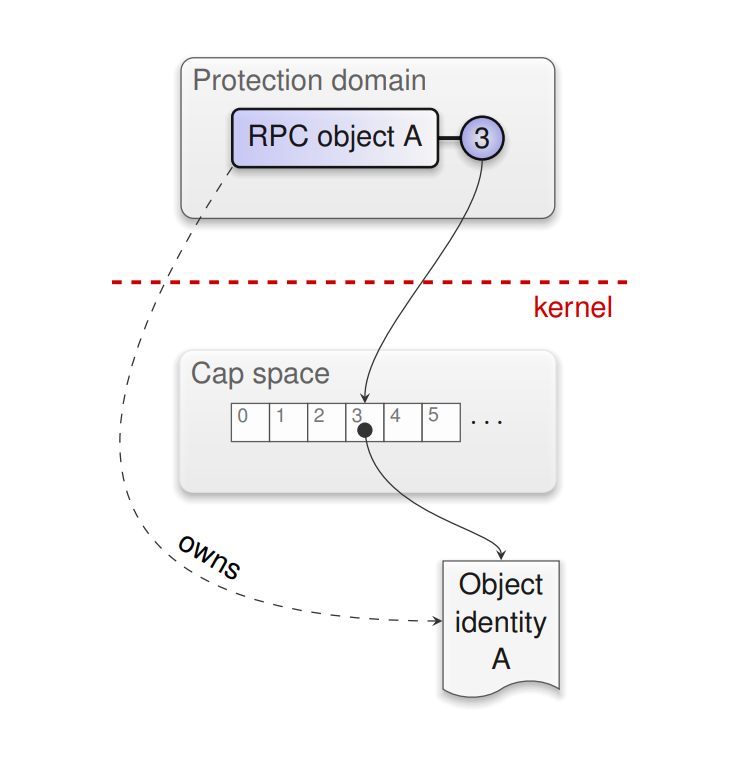
\includegraphics[width=0.5\textwidth]{Images/Cap_space.PNG}
    \caption{Relationship between an RPC object and its corresponding object identity. \cite[P.41]{genode_foundations}}
    \label{fig:Cap_space}
\end{figure}
\subsubsection{Capability Delegation}
Finally the question of how RPC objects can be accessed from other components remains. This is solved by sharing capabilities through the concept of delegation. Similarly to aforementioned pointer, a capability can be passed to another component, with which the associated RPC object can then be evoked. These delegated capabilities each index an element in the capability space of the component it was delegated to, but these elements in turn point to the same object identity. The concept of delegation, which is illustrated in figure \ref{fig:delegation}, is essential for purposes of any inter-component communication, and therefore represents a backbone of the entire architecture. \cite[P.41-42]{genode_foundations}
\begin{figure}
    \centering
    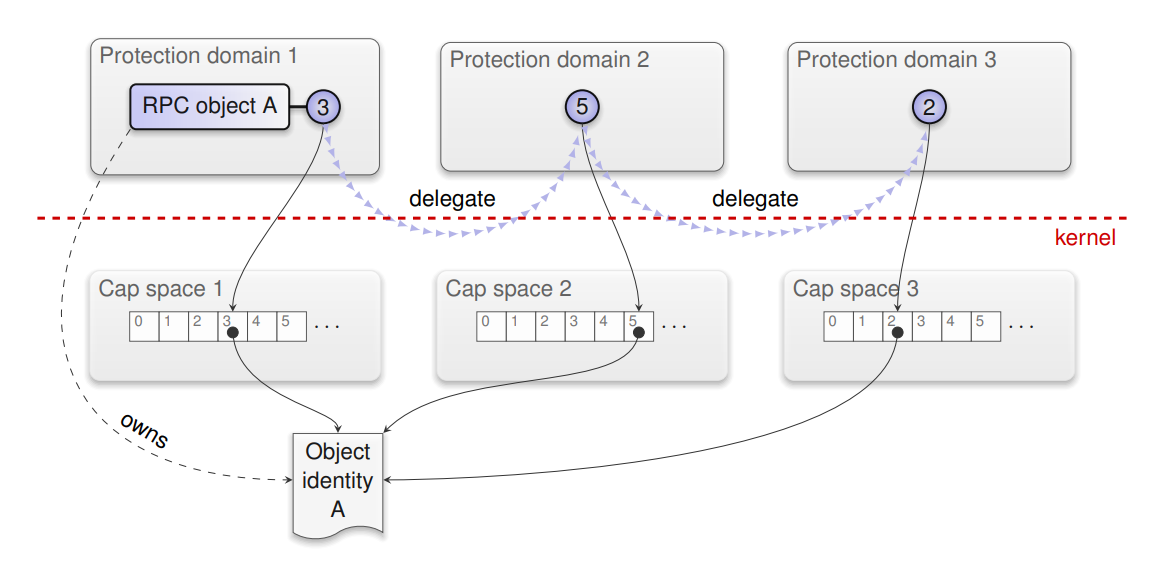
\includegraphics[width=0.75\textwidth]{Images/delegation.PNG}
    \caption{The transitive delegation of a capability from one protection domain to others. \cite[P.42]{genode_foundations}}
    \label{fig:delegation}
\end{figure}
\subsection{Recursive System Structure}
The last section introduced the fundamental parts of the Genode architecture, but what remains to be explained is how these components are connected to each other. The overall system structure is a tree of components, where every component except the root of this tree has a parent. This root is called core and it has access to the raw physical resources, which it then distributes to other components as capabilities to RPC objects. These RPC objects that interface the physical resources are:
\begin{itemize}
    \item Dataspaces: A dataspace is the representation of a physical address-space region of any size.
    \item Region maps: A region map is the layout of a virtual address space. Similarly to how a MMU populates page tables with physical page frames, a region map is populated with dataspaces. One dataspace can therefore be attached to multiple region maps.
    \item Access to boot modules (ROM): These RPC objects represent different binaries initially loaded into the memory by the boot loader, which are then made available as read-only memory to clients. 
    \item Protection domains (PD): A protection domain defines the boundaries of a component within the Genode system, where typically one PD corresponds to one component. Each PD consists of three region maps, a capability space, and a physical memory and capability budget.
    \item Region-map management (RM): The RM service allows components to allocate more than the aforementioned three region maps.
    \item Processing-time allocation (CPU): The CPU service can be used to create, control and terminate threads.
    \item "Device resources (IO\_MEM, IO\_PORT, IRQ): Core’s IO\_MEM, IO\_PORT, and IRQ services enable the realization of user-level device drivers as Genode components." \cite[P.69]{genode_foundations}
    \item Logging (LOG): The LOG service allows components to print diagnostic output.
    \item Event tracing (TRACE): The TRACE service is a non-fundamental light-weight event-tracing facility.
\end{itemize}
\cite[P.65-71]{genode_foundations}

\subsubsection{Client-Server Relationship}
To now establish a connection between a component offering a service (server) and another component that wants to use this service (client), a multitude of actions have to be performed. This is explained using the example of a GUI component as a server, offering a GUI service, and an application, which represents the client. Firstly, the GUI component has to announce its service to its parent using its parent interface, which is a capability to the parent RPC object that was delegated to it at creation time. Announcing is done by delegating a capability to the service root RPC object. 

On the other side, the application requests a GUI session from its parent interface. These requests are passed up the tree until it reaches the parent of the GUI component, which uses its capability to the root RPC object to create a session RPC object. A capability to that session RPC object is then passed to the initial caller. Figure \ref{fig:client-server} shows the setup after the final delegation was made. 

It is important to highlight that due to the parent having complete control over both the sessions established within the child on server side and requests done by the child on client side, security is further improved. \cite[P.50-54]{genode_foundations}
\begin{figure}
    \centering
    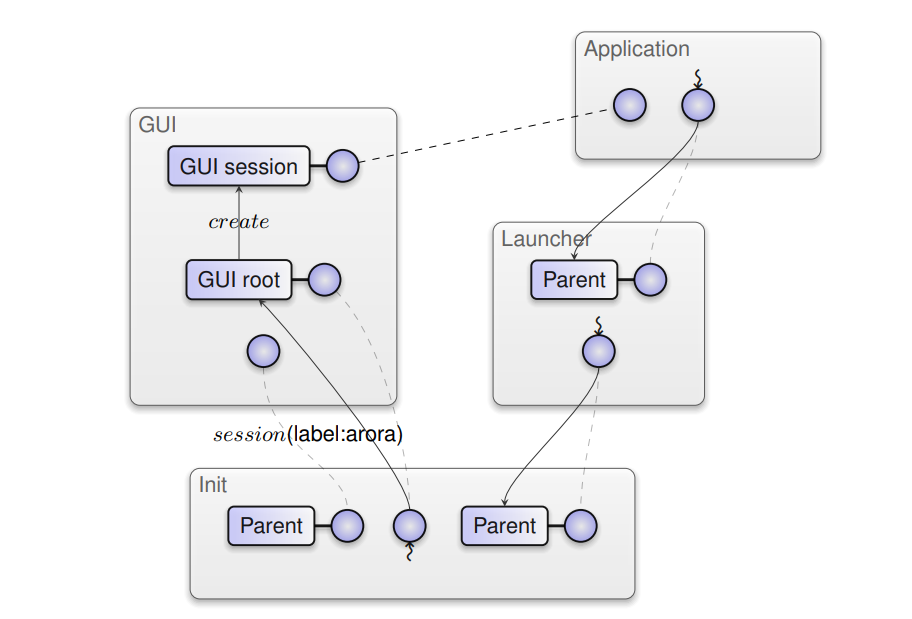
\includegraphics[width=0.75\textwidth]{Images/client-server.PNG}
    \caption{Example of client-server relationship after final session delegation. \cite[P.52]{genode_foundations}}
    \label{fig:client-server}
\end{figure}
\newline
\newline
Within an actual project, a session interface defining the RPC functions needs to be created as the first step. This interface is implemented inside a session component object by the server, which can be created by the server's parent because the servers root component was announced to it, handing it the capability. 

To implement a complete client, a session client class which takes a session capability in its constructor and implements the RPC interface for the client, has to be declared. The remaining issue now is how a session client object would obtain the necessary capability. The solution being a wrapper called a connection object, which inherits from the session client. This object is responsible for issuing a session request to the parent and retrieving the capability, with which a session client object can be created. Because of this preparatory work the client side implementation is straightforward: it simply declares a connection corresponding to the service that it wants to use and calls functions on it as if it were a session client object. A simplified illustration of the classes making up this functionality can be seen in figure \ref{fig:client-server_classdiagram}. \cite{client-server_tutorial}
\begin{figure}
    \centering
    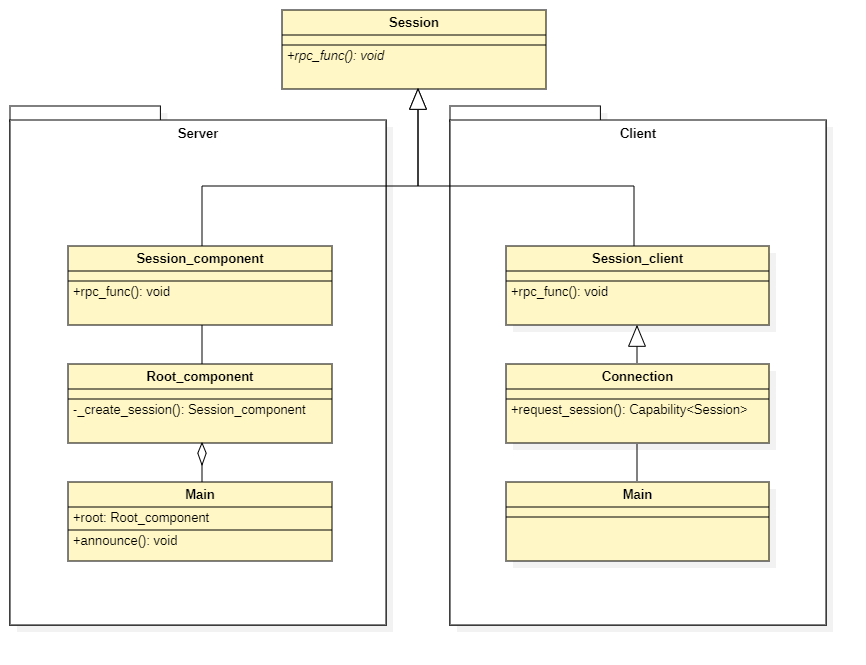
\includegraphics[width=0.7\textwidth]{Images/client-server_classdiagram.png}
    \caption{Class diagram of the components making up the client-server infrastructure.}
    \label{fig:client-server_classdiagram}
\end{figure}

\subsection{Networking in the Genode OS framework}\label{subsection:network}
Since the checkpoint management system has to be able to communicate with other components across ECU boundaries, the network stack comes into play. In Genode, most user-level network communication is done using the socket API, which is handled by a lightweight TCP/IP stack called lwIP. The network stacks of the different components then access a network interface controller session provided by a NIC-router, which acts as a multiplexing component so that the applications do not directly operate on the actual network drivers, allowing the use of the networking interface by multiple applications.

Instead of having the NIC-driver delegate a session to the NIC-router, as was generally the case until Genode version 21.02, the driver acts as a client towards the router by using a so-called uplink session, provided by the latter. This architectural change was implemented because the NIC driver was deemed too fragile due to its high complexity, leading to the lifetime of an application being put at risk by being bound to it. The structure is depicted in figure \ref{fig:network_architecture} with the additional underlying components of platform driver, core/init, and the kernel. \cite{nic}

\begin{figure}
    \centering
    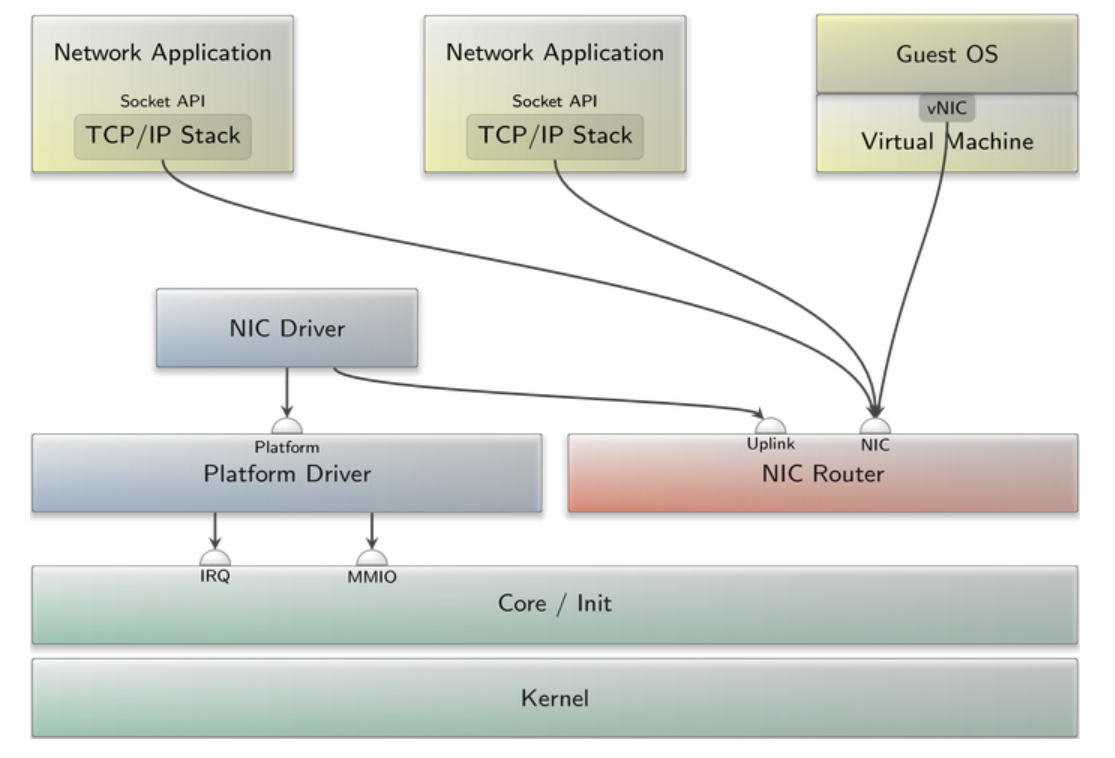
\includegraphics[width=0.7\textwidth]{Images/network_architecture.png}
    \caption{Visualisation of the Genode OS network architecture after Genode 21.02. \cite{nic}}
    \label{fig:network_architecture}
\end{figure}

\section{Distributed Shared Memory for Genode}\label{section:DSM}
The development of a checkpoint management system necessitates data transfer between components running on different ECUs. One way to accomplish this and possibly answer the research question regarding receipt of checkpoints is by a distributed shared memory (DSM), of which a prototype was developed by Weidinger in 2016 for Fiasco.OC/Genode OS 15.02.

The main functionality of establishing and updating the shared memory is handled by two broker components which are spawned by the processes that wish to share memory across system boundaries. These brokers first establish a local shared memory by delegating a capability to the dataspace and then detect read and write accesses to the memory on their respective sides by the handling of page faults, which triggers the sending of data to the other system over Ethernet using TCP/IP. It is important to note that because of the local shared memory, the DSM functionality is completely transparent to both processes. 

However, the consistency module, which checks if both dataspaces representing the shared memory are identical and is an essential aspect of an DSM is not implemented. \cite{dsm}
% !TeX root = ../main.tex
% Add the above to each chapter to make compiling the PDF easier in some editors.

\chapter{Concept}\label{chapter:concept}
The following chapter presents the main aspects of a checkpoint management system (CMS), and how these functionalities could be realised. For each aspect a decision is made, resulting in a complete conceptualisation.
\section{Location}
The first issue is the location of the manager. There are two main approaches for this. One would be to have a single checkpoint manager running on every ECU, which is responsible for the checkpoints generated by the RTCR on its respective machine, and the other is one CMS component which manages the entire system. In the former approach, on ECU breakdown, another manager would then need to be selected through communication between every manager to retrieve the checkpoint and restore it on its own ECU. This star topology communication, and the fact that such a system would make more sense integrated into RTCR, makes this approach unfeasible. 
The latter, more sensible solution, would be a centralised management system which receives checkpoints from the RTCR components on their respective ECUs is proposed. This manager both stores the checkpoints and is responsible for their migration and restoration on another system. This however marks a single point of failure in the entire infrastructure, reducing system resilience and therefore rendering the manager useless. Thus redundancy is used in the form of at least two checkpoint management systems running on different ECUs and performing identical tasks. 
\section{Receiving of Checkpoints}
The next key question to be answered is how the manager gains access to the checkpoints made by RTCR. For this, three possible solutions are compared.
\subsection{Publish/Subscribe}
The first thing that comes to mind to resolve the issue of sending checkpoints on the side of the RTCR and receiving them on the side of the CMS is a simple publish and subscribe system. Here, all instances of RTCR connect to an interface set up by the manager and then send checkpoints over Ethernet whenever a new one is created. This approach is commendable for its simplicity of both concept and implementation, but has a couple of flaws: first being due to the redundancy of management systems, the manager is not transparent to the RTCR, because checkpoints have to be sent to every instance of the checkpoint manager. Another major problem is that for many RTCR components which in turn manage many components, lots of network traffic in form of checkpoints is sent to only one interface of the centralised checkpoints management system. This will quickly lead to network congestion. Therefore a solution where the CMS can receive checkpoints at its own pace is desired and presented in the following subsection.
\subsection{Distributed Shared Memory}
The DSM implemented by Weidinger, which was presented in section \ref{section:DSM} is the obvious choice for this approach. It makes it possible to exchange checkpoints between one RTCR instance and the at least two redundant instances of CMS transparently, since the RTCR theoretically never directly has to address the CMS. The missing consistency module of Weidinger's DSM doesn't present an issue here, as the RTCR would be the only component writing into the shared memory. In the possible case of CMS and an instance of RTCR operating on the same ECU, a simple shared memory utilising Genode dataspace capabilities is used. The RTCR checks for this when it attempts to establish the DSM, and in case it resides on the same ECU, the RPC interface is used.

Once the DSM is established, the CMS would then have to monitor the dataspace and store a checkpoint to their own memory whenever a change is detected. Unfortunately this kind of detection is not feasible, as the CMS itself never has direct access to the memory the RTCR writes to. Two possibilities of resolving this issue are described. Firstly, there is the naive solution of serialising and downloading all new checkpoints at set intervals. The advantage of this approach is its simplicity, but it suffers heavily from the chance of increasing checkpoint age when having to fallback farther than the granularity of the RTCR checkpointing interval. Mitigating this issue by increasing the interval entails massive network load, as a whole array of checkpoints is downloaded frequently. The second solution, a hybrid between the approaches publish/subscribe and the DSM is presented in the following section.
\subsection{Hybrid}
In this solution the receipt of checkpoints does not rely on downloading intervals. Here the RTCR broadcasts a notification whenever it writes a new checkpoint to its shared memory, containing the memory address of the updated checkpoint. The CMS can then use the IP-address from the IP-header, finds, serialises, and downloads the checkpoint in a newly spawned thread. The advantage of this approach is that it resolves all disadvantages of the naive “downloading at intervals” solution. Therefore, it would seem like the obvious choice, however one caveat exists: To maintain transparency of the redundant managers, every RTCR has to broadcast a small amount of data whenever a checkpoint is made, perhaps containing sensitive information. For many RTCRs handling many components the volume of messages might overload the network. This is only an issue for the current concept, as it would be resolved whenever the DSM functionality is integrated into is participants: due to this integration, the RTCR knows the IP-addresses of its participants, and can thus replace the broadcast with a multicast. Transparency suffers due to this hybrid solution, but overall is deemed negligible, as the addresses of the checkpoint management systems are only used for this single multicast, which can be implemented in a completely flexible fashion concerning the number of redundant checkpoint managers. Furthermore addressing the management systems is necessary in scope of migration and restoration anyway, as outlined in the eponymous section. 
\newline \newline
Altogether, the decision has to be made in favour of the hybrid solution, as it unites the positives of both the publish/subscribe and DSM approaches, with only a few drawbacks remaining.
\section{Checkpoint Storage}
After receipt of the checkpoints, the next step is to store them securely. The best way of achieving this and avoiding the vulnerability of local checkpoint storage, would be to have both management systems store them on the same network addressed storage in RAID configuration. The possibility of single point of failure is resolved due to the storage being configured in RAID, which enables both the main and the redundant system to write to the same memory. Therefore it is not necessary to integrate two network addressed storages into the infrastructure.

For purposes of efficient retrieval, the CMS and NAS have to define a primary key identifying a checkpoint uniquely. The decision for this key was made in favour of a combination of MAC-address and memory offset of the checkpoint on the machine it originated from. The MAC, offset, and serialised checkpoint will then be composited into an object containing all the necessary information. Figure \ref{fig:store_activity} depicts the control flow of storing such a checkpoint.
\begin{figure}
    \centering
    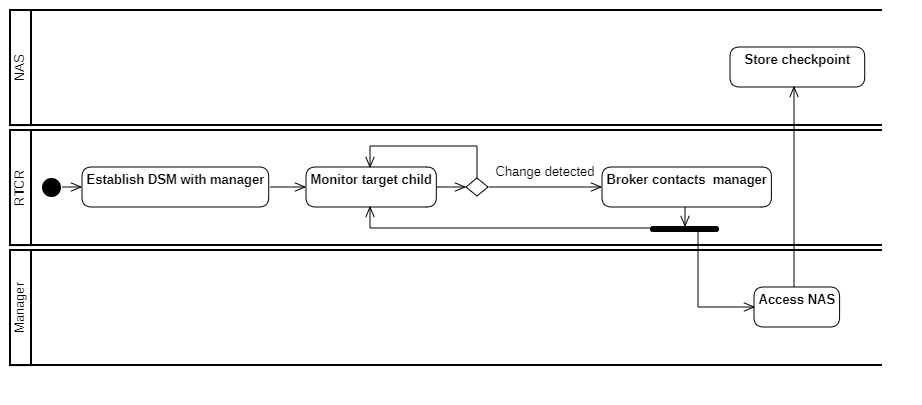
\includegraphics[width=\textwidth]{Images/checkpoint-storing_activity.png}
    \caption{Activity diagram visualising storing of checkpoints.}
    \label{fig:store_activity}
\end{figure}
\section{Migration and Restoration}\label{section:Migration_and_Restoration}
There are two different scenarios where migration and restoration is necessary. The first being when one of the RTCR components asks the CMS to migrate and restore one of its programs, for example for load balancing reasons. In this case the MAC-address and offset of the checkpoint have to be transmitted. The CMS then retrieves the serialised checkpoint from memory and selects the ECU to restore it on.

The second case is that the ECU or the RTCR thereon stops working entirely. For this purpose, it is assumed that the CMS knows of the event and the MAC-address of the board it occured on. All checkpoint objects with that MAC-address are then retrieved and restored one by one on another selected machine.
The selection for both scenarios is made by comparing the ECUs in the network using different performance metrics. These metrics are
\begin{itemize}
    \item CPU load
    \item RAM usage
    \item Capability quota
\end{itemize}
of the ECU. Since this information is not accessible over network through any already existing Genode interface, the RTCR has to provide such an interface, whereupon demand it accesses CPU load, RAM usage, and capability quota locally.

One big issue is that the redundancy of managers warrants that they have to agree upon which component performs the restoration and thereby avoid duplicate processes. As timing differences of the managers might make one ECU more or less suitable than it was at migration time of another checkpoint manager, the possibility of them restoring the checkpoint on different platforms has to be acknowledged. The decision is therefore made at the time of checkpoint retrieval. Whichever is the first to access a checkpoint from the NAS, is the one to migrate and restore the checkpoint. This is enforced by a mutex and the immediate deletion of the checkpoint from the database. This is necessary in any case, as both offset and MAC-address are those of the old host of the process and therefore expired. 

The entire process of migration and restoration is shown in figure \ref{fig:migr_activity}.
\begin{figure}
    \centering
    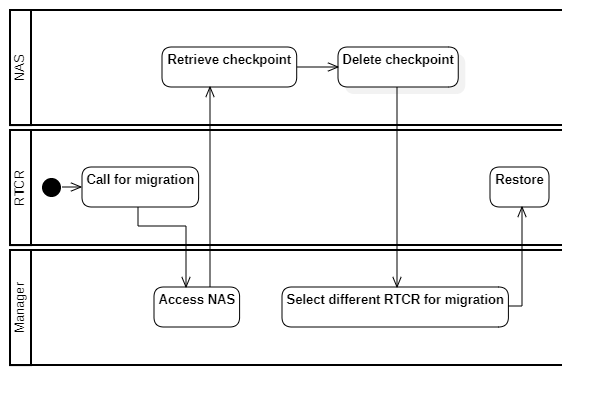
\includegraphics[width=0.75\textwidth]{Images/migration-restoration_activity.png}
    \caption{Activity diagram visualising migration and restoration.}
    \label{fig:migr_activity}
\end{figure}
\section{Considerations outside of Implementation Scope}
The following sections touch on aspects of a checkpoint management system, that are important to consider given its foundations, but were deemed too time-intensive to be within the scope of the implementation.
\subsection{Knowing a Restoration is Necessary}
For the CMS to provide failure safety while still avoiding redundant inactive ECUs, it needs to know that either the ECU itself or the RTCR component failed. The naive solution is to implement heartbeats into every single RTCR component, which are then checked by the CMS. If the heartbeat from an ECU stops, a migration and restoration is performed. This approach can be either accomplished with the RTCR multicasting a heartbeat to the managers or with the CMS requesting a heartbeat from an RTCR interface, both with a set interval. These solutions heavily utilise the network and therefore put it under unnecessary load. Fortunately, the architecture of KIA4SM provides a more sensible resolution: because of the homogeneity of ECUs and the resulting possibility of any process running on any ECU, some sort of meta-entity has to exist, which distributes the processes to their systems at the beginning, and later schedules them. Such an entity would also be responsible for notifying the manager of system failures.

\subsection{Managing Checkpoints in Real Time}
An important aspect of RTCR is its real-time capability, which warrants a discussion concerning the real-time capability of the system managing the RTCR instances, even though it is not part of the practical implementation. There are two aspects that may hinder the target child at fulfilling its schedules. One of them is the obvious loss of time of needing to migrate and restore the program, which has to be mitigated by increasing performance of migration and restoration, maybe by even using hardware-assisted solutions. The other aspect is the schedule on the machine that is being migrated to. If many programs with real-time demand are already in execution, the scheduler on the new ECU might have to enforce that our program misses a schedule. Resolving this completely would entail knowing the state of the scheduler on any ECU that is eligible for migration. However an estimate can be made using CPU load and RAM usage, which is already included in the current concept of ECU selection. Ultimately, both an interface providing information about current schedules on the side of RTCR and a complex module parsing this data and making decisions based on it are required.
% !TeX root = ../main.tex
% Add the above to each chapter to make compiling the PDF easier in some editors.

\chapter{Implementation}\label{chapter:implementation}
After discussing the concept of a checkpoint management system, this chapter focuses on the actual implementation of a prototype in C++ utilising the API of Genode version 21.08. 
\section{Run-Script}
"The Genode OS Framework comes with a custom build system that is designed for the creation of highly modular and portable systems software." \cite{build_system} This build directory targets a specific platform, in our case the Fiasco.OC microkernel and the RealView PBX-A9 hardware architecture. From within these directories system scenarios are executed via their run-script, a file responsible for building the components, creating a boot directory, configuring the init process, creating a bootable system image, and finally executing the system image. \cite{build_system}
This script is essential to the system scenario executed, and therefore important aspects and how they were implemented, are presented.
\subsection{Package Management}
The advantages of the run tool are automation of building, configuration, integration and testing. This results in one image with a certain set of features. If any part of the automated chain changes, a completely new image has to be created, which means having to recompile all components during the process of building. For complicated system scenarios with many components, this induces an unnecessary overhead. The concept of depots aims to resolve this issue: archives are downloaded preemptively and then imported by the run script. \cite{package_management} The following listing shows the code used for the building part of the \verb|manager.run| script, which executes the system scenario of the checkpoint management system.

\begin{lstlisting}[caption={Importing of depot archives and subsequent building in manager.run.}]
import_from_depot [depot_user]/src/[base_src] \
                  [depot_user]/pkg/[drivers_nic_pkg] \
                  [depot_user]/src/nic_router \
                  [depot_user]/src/init \
                  [depot_user]/src/libc \
                  [depot_user]/src/vfs_lwip \
                  [depot_user]/src/vfs \
                  [depot_user]/src/stdcxx

build { manager rtcr_dummy nas}
\end{lstlisting}
\verb|[depot_user]| stands for the origin of the archives contained within the directory, as it is possible to download an archive with an identical name to the archive of another user. \verb|[base_src]| refers to the base archives corresponding to the selected microkernel and hardware architecture. The \verb|nic_router| archive together with the NIC-drivers package is responsible for the network interface, which architecture was explained in section \ref{subsection:network}. The socket API that uses lwIP is integrated into the libc library, which depends on the virtual file system (vfs). These archives are therefore also imported. Of the two remaining archives, \verb|init| represents the initial component serving as a parent to the components making up the system scenario, while \verb|stdcxx| is a library containing the C++ standard library ported to Genode OS.

Ultimately, only the manager, rtcr\_dummy and nas components have to be compiled and built with every execution, with all components that don't change being imported as archives, significantly reducing the overhead.
\subsection{Configuration of the Init Component}
Init is the component which controls the execution of all further components making up the system scenario. The policy of init is defined by configuring it and all its children together with the services they require and provide inside an XML config in the run-script. Within the root config tags, the services provided by init's parent core, like ROM, IO\_MEM and CPU, and the concrete components of the system scenario are listed. In our case, outside of the manager, RTCR and NAS programs, this also includes the timer, drivers and nic\_router components. After presenting and explaining the configuration of the main components, their interplay through the nic\_router and its configuration, is also shown. \cite{init_config}
\subsubsection{Main Components}
The basic elements of a component configuration are its name, its RAM and capability quotas, the services it provides to other components, and a routing table to services that are being offered by others. If RAM or capability quotas are not stated explicitly, the component is configured with a default quota defined in the configuration of init. The following listing shows the manager definition, where name, quota and the provided service called "Manager", which is utilised when RTCR and manager are on the same ECU, are self-evident. In the system scenario making up the prototype, only one manager without any redundant components is employed, because integrating and testing another manager into the system was too time-intensive. The routing table can be found within the \verb|<route>| tags. Here the route to the "Nic" service is stated by pointing to the nic\_router component, whereas for all other services, a default route pointing to init's parent or any other child of init is utilised. \cite{init_config}
\begin{lstlisting}[language=XML, caption={Configuration of the manager component.}]
<start name="manager">
    <resource name="RAM" quantum="10M"/>
    <provides> <service name="Manager"/> </provides>
    <config port="1024" nas_ip="10.0.2.2" nas_port="1027" rtcr_info_port="1025" rtcr_migr_port="1026">
        <vfs>
            <dir name="dev"> <log/> </dir>
            <dir name="socket">
                    <lwip ip_addr="10.0.0.2"
                          netmask="255.255.255.0"
                          gateway="10.0.0.1"/>
            </dir>
        </vfs>
        <libc stdout="/dev/log" stderr="/dev/log" socket="/socket"/>
    </config>
    <route>
		<service name="Nic"> <child name="nic_router"/> </service>
		<any-service> <parent/> <any-child/> </any-service>
	</route>
</start>
\end{lstlisting}
The remainder is necessary information for networking and diagnostic printing. Directly within the \verb|<config>| tags, the static ports and IPs of certain services provided over Ethernet are defined. Because the configuration is provided to the components as a ROM-session, it is possible to read from these definitions from within the actual implementation and thus prevent hard coding numbers. These ports and services are:
\begin{itemize}
    \item 1024: The port through which messages to the manager's main interface are handled.
    \item 1025: The RTCR provides an interface for system information to allow the manager to decide where to migrate a checkpoint to on this port.
    \item 1026: Checkpoints sent to this port are restored under the RTCR running on the respective ECU.
    \item 1027: This port is where the NAS handles both checkpoint storage and retrieval requests.
\end{itemize}
Another important element that has to be configured is the virtual file system (VFS), as libc depends on it, and the socket API we wish to use relies on libc. In Genode, file systems are component-local. Therefore each component that uses the VFS has its own root directory, from which the file system structure is spanned. Inside the \verb|<vfs>| tags this structure can be customised with any conceivable directories or files, but in this case two conventional directories are introduced to the file system of the manager component. Firstly, the directory "dev" is added, within which the \verb|<log/>| file-system plugin adds a file called \verb|log|. This file forwards everything written to it to the Log session of the program.
Inside the second directory named "socket", the IP-stack plugin \verb|<lwip/>| configures the network stack with an IP-address, a netmask and a standard gateway.

Finally libc itself is also equipped with standard outputs and a socket interface by declaring the environment variables \verb|stdout|, \verb|stderr| and \verb|socket|, using the previously defined file system structure. \cite{vfs_basics} \cite{vfs_networking}
\newline \newline
The other main component besides the NAS, of which the configuration is very similar to that of the manager and therefore not further presented, is the RTCR. However, because it would have to be ported to the current version of Genode, a dummy is employed. The configuration of one such RTCR-dummy is shown in the following listing. For reasons of testing, the system scenario is equipped with two RTCR-dummies with different names using the same source code. This step is evident by the additional \verb|<binary>| tag, which contains the name of the source binary. Another difference is that the routing table additionally points to the service offered by the manager component.
\begin{lstlisting}[language=XML, caption={Configuration of one of the two RTCR-dummy components.}]
<start name="rtcr_dummy_1">
    <binary name="rtcr_dummy"/>
    <resource name="RAM" quantum="10M"/>
    <config name="dummy_1" ip="10.0.1.2" mac="57406533673528" manager_ip="10.0.0.2" manager_port="1024" info_port="1025" migr_port="1026">
        <vfs>
            <dir name="dev"> <log/> </dir>
            <dir name="socket"> <lwip ip_addr="10.0.1.2"
                                      netmask="255.255.255.0"
                                      gateway="10.0.1.1"/>
            </dir>
        </vfs>
        <libc stdout="/dev/log" stderr="/dev/log" socket="/socket"/>
    </config>
    <route>
		<service name="Nic"> <child name="nic_router"/> </service>
	    <service name="Manager"> <child name="manager"/> </service>
		<any-service> <parent/> <any-child/> </any-service>
	</route>
</start>
\end{lstlisting}
The config section of the RTCR-dummy is very similar to the manager, except the extra variable definitions for name, IP- and MAC-address of the component. This seemingly superfluous information is necessary, because no way was found to determine these values dynamically from the component name in the first, and from the network stack in the last two cases. The name is required for diagnostics, while IP and MAC need to be transmitted to the manager for purposes of RTCR interface access and identification, respectively. Here the MAC is saved as an 48 bit integer, which translated into conventional notation is 52:54:00:12:34:56. The IP- and MAC-addresses of the second RTCR-dummy are those of the first incremented by one.
\subsubsection{Nic\_router}
To ultimately enable the components to communicate using their respective network stacks, a mediation unit is required. This mediation unit is the NIC-router, as presented in section \ref{subsection:network}. With this unit in play, the system scenario closely resembles two applications on different ECUs connected through a real router, as is conceptualised. The configuration of the router is shown in the following listing.
\begin{lstlisting}[language=XML, caption={Configuration of the NIC-router component.}] 
<start name="nic_router" caps="1000">
    	<resource name="RAM" quantum="32M"/>
	<provides>
		<service name="Nic"/>
		<service name="Uplink"/>
	</provides>
	<config>
	    <policy label_prefix="drivers" domain="uplink"/>
		<policy label_prefix="manager" domain="manager"/>
		<policy label_prefix="rtcr_dummy" domain="rtcr"/>
		<policy label_prefix="nas" domain="nas"/>

		<domain name="uplink">
			<nat domain="manager" tcp-ports="100"/>
			<nat domain="rtcr" tcp-ports="100"/>
			<nat domain="nas" tcp-ports="100"/>
		</domain>
		<domain name="manager" interface="10.0.0.1/24">
		    <tcp dst="10.0.1.0/24">
		        <permit port="1025" domain="rtcr" />
		        <permit port="1026" domain="rtcr" />
		    </tcp>
		    <tcp dst="10.0.2.0/24">
		        <permit port="1027" domain="nas" />
		    </tcp>
		</domain>
		<domain name="rtcr" interface="10.0.1.1/24">
			<tcp dst="10.0.0.0/24">
			    <permit-any domain="manager" />
			</tcp>
		</domain>
		<domain name="nas" interface="10.0.2.1/24">
		</domain>
	</config>
</start>
\end{lstlisting}
As presented in section \ref{subsection:network}, the NIC-router provides two services: the "Nic" service to the network stacks of the components and the "Uplink" service to the network driver. The config section is split into policies which are differentiated by a prefix of the component name. These policies then direct the traffic into domains with corresponding interfaces, where router rules can be applied. The "rtcr" domain for example permits all traffic targeting any port as long as its destination is in the domain of the manager. The "rtcr" domain is configured this way, because the manager dynamically allocates ports and then forwards them to RTCR for purposes of DSM establishment. In contrast, the "manager" domain drops all packets not directed at specific ports within the "rtcr" or "nas" domain, as these ports are always the same for their respective services. \cite{nic_readme}

\subsection{Execution}
The execution of the system scenario is the last action carried out by the run-script. To simulate a real scenario as closely as possible, QEMU is first set up and then used as the system on which to run on. After configuring the NIC-model the correct parameter depending on the processor architecture, \verb|run_genode_until forever| is executed, to self-evident effect.

\section{Manager Component}
This section presents the main component of the system scenario, the manager. After being constructed, it enters its main routine, where it offers its main interface on port 1024, using the libc socket API. As described in the section regarding the run-script, the values of static ports and IPs are imported to the program using an \verb|Attached_rom_dataspace| and reading from it as an \verb|Xml_node|. Furthermore, a root component is started and announced to its parent, allowing instances of RTCR to connect if they are on the same ECU, using RPC interfaces almost identical to the ones reachable over Ethernet. For both of these interfaces, after handling the parameters sent by the client, the same subsystems are executed, resulting in a facade design pattern with two different facades, where only one is reachable by any client at the same time. The distinction whether the RTCR is to use the socket or the internal interface should be decided by the RTCR by comparing IP addresses. The focus of this section lies on the interface reachable over Ethernet, as this is more likely to be accessed and could be tested more comprehensively. The only real difference between the two, is that for internal communication simple parameter passing is utilised, whereas when using the socket interface of the manager, a certain message format is expected, which is depicted in figure \ref{fig:main_message_format}. The first twelve bytes contain MAC and IP of the ECU of the RTCR needing to either establish a DSM, notify of a new checkpoint or call for a migration. These parameters don't necessarily have to be the values of the message author, but are so in most cases. The content of payload and opcode, labeled "Op" in the figure, depend on the desired functionality. These and their corresponding values are presented in the following three sections.
\begin{figure}
    \centering
    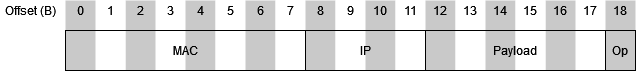
\includegraphics[width=\textwidth]{Images/main_message_format.png}
    \caption{Message format expected on the main manager interface.}
    \label{fig:main_message_format}
\end{figure}
\subsection{DSM Establishment}\label{subsection:DSM_establishment}
The desire to establish a DSM with the manager is expressed with an opcode of zero. In this case the first four bytes of the payload are reserved for the size of the shared memory, while the remaining two are set to zero. The decision of how large the DSM has to be, should be made by the RTCR, where considerations like number of protected processes and size of the checkpoints of these processes influence the size required. The first action the manager undertakes is to select a port on which this new DSM is to be established. The chosen solution for this is to increment through the ephemeral ports starting at 1025, as 1024 is already in use. The maximum possible port would then be 65535. It is unlikely that such a high amount of RTCRs wish to establish a DSM, therefore wraparounds are deemed to be irrelevant. Afterwards, the manager allocates the memory and passes start address, size and the selected port to a new POSIX-thread named "Broker\_thread", which currently only sets up a server to receive checkpoints and store them to the allocated memory, simulating a DSM. The DSM by Weidinger could not be used, as it was implemented for Genode 15.02, necessitating large porting efforts to get it to function on the current Genode version. 

On the side of the RTCR, after receiving the port the manager wants it to connect to, a thread also called "Broker\_thread" is spawned, which sends the first checkpoint when it first connects to the broker of the manager. This message contains the offset of the checkpoint in the memory of RTCR within the first four bytes, the size of this checkpoint within the next two bytes and then the actual checkpoint. On receipt by the broker thread of the manager, this checkpoint is then written to the previously allocated memory at the specified offset. It has to be remarked that the current size of the buffer which the checkpoint is written to during network relay is set to 1024 bytes. This value needs to be modified according to the maximum size of a serialised checkpoint.

Meanwhile the main thread of the manager inserts the MAC, IP and address of the memory shared with the RTCR running on the ECU identified by the previous two parameters to a map it maintains. This map is necessary to be able to access the correct memory and store a checkpoint when notified by an instance of RTCR using the address and later iterate over when choosing an RTCR to migrate to by contacting the interfaces using the stored IP-addresses. The remaining value, the MAC, is used as the primary key.

The next step is for the RTCR to notify the CMS, that this checkpoint was sent to its memory by utilising the next functionality, described in the following section.
\subsection{Storing of Checkpoints}
An opcode of one in a message sent to the main manager interface means that a new checkpoint was just sent to the broker and written to memory. In this case the entire six bytes of payload are utilised: the first four bytes are for the offset of the checkpoint in the "shared" memory, whereas the last two bytes represent the size of the checkpoint. Together with the information of where the memory resides on the machine of the manager, which it retrieves from the previously mentioned map using the MAC as key, the checkpoint can then be read and sent to the network addressed storage. This process is accomplished by another POSIX-thread, so that the main thread of the manager can return to its server functionality as quickly as possible. The thread receives the necessary information to connect to the NAS, i.e. IP and port, and the previously mentioned values of offset, size, MAC-address and map as passing parameters. The combined process of connecting to the manager, establishing a pseudo DSM, and subsequently storing a checkpoint is further visualised in a sequence diagram in figure \ref{fig:dsm-and-store_sequence}.
\begin{figure}
    \centering
    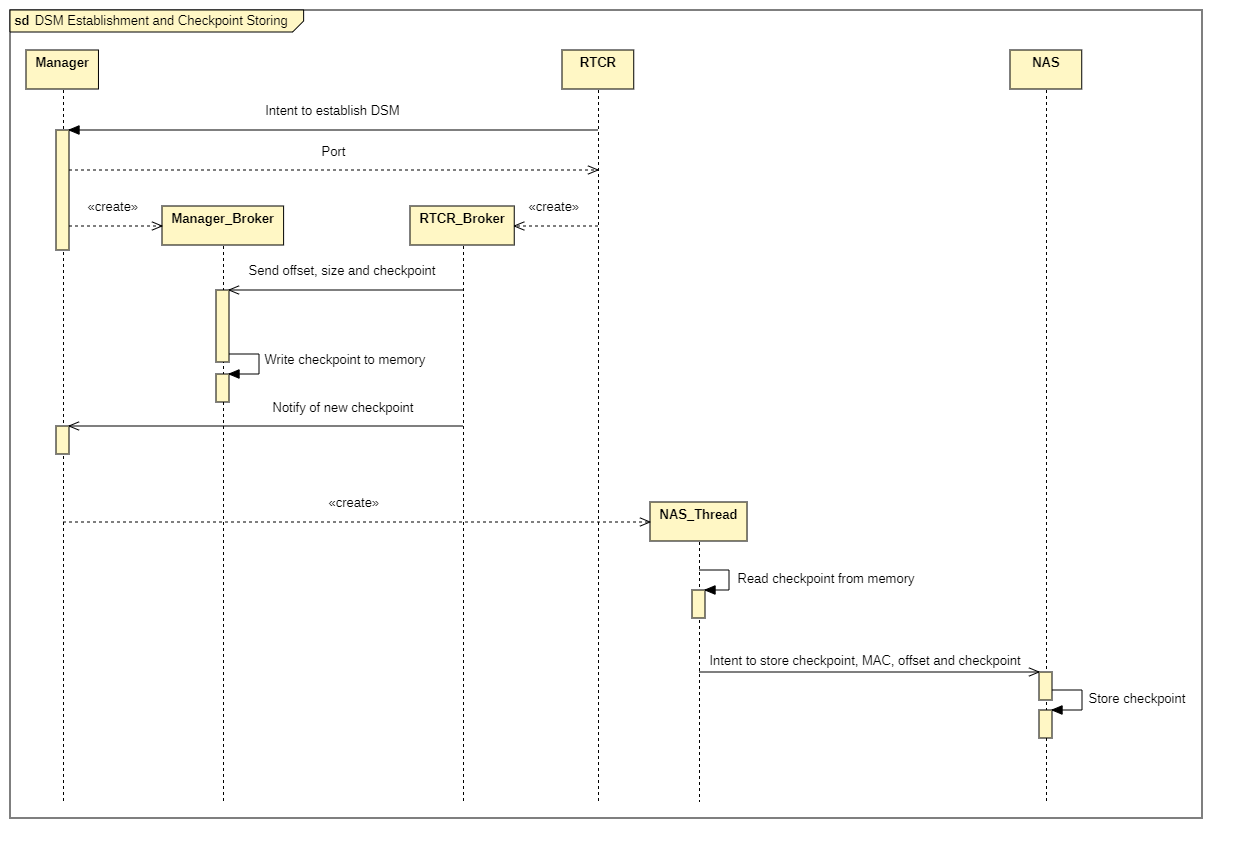
\includegraphics[width=1.25\textwidth, angle=90]{Images/dsm-and-store_sequence.png}
    \caption{Sequence diagram showing the establishment of a pseudo DSM and storing of a new checkpoint.}
    \label{fig:dsm-and-store_sequence}
\end{figure}
\subsection{Migration and Restoration}
A call for migration and restoration is stated by contacting the manager with an opcode of two. Hereby the payload of the message is used for the offset of the checkpoint, which together with the MAC address, uniquely identifies it. Resembling the interface for notification about a new checkpoint, the first four bytes are used for the offset, while in contrast to the aforementioned interface, the last two bytes remain unused. Another similarity is that a POSIX-thread is spawned to handle the actual process, again for the server to return to the beginning of its loop. This thread then performs the tasks of selecting a target to migrate to, retrieving the checkpoint from the NAS, and ultimately restoring it. The first task relies on an interface provided by the RTCR, as described in section \ref{section:Migration_and_Restoration}. However, no solution to the problem of determining CPU usage was found, resulting in only two parameters being prompted: available RAM and available capabilities. Both of these values are immediately sent to the client on connection to the socket always reachable on port 1025. Afterwards, the thread on the side of the manager creates a metric by multiplying the two parameters. As the available RAM is given in bytes, it is usually a much larger number than the remaining capabilities, making it the determinative parameter of the equation, but not as determinative as if the values where simply added. The behaviour of RAM being more important, but not so important, that an ECU with zero available capabilities could possible be selected for migration, is desired. The choice of metric in favour of multiplication was made due to this reason.

All to the manager known RTCRs, except the one calling for migration, are contacted by iterating over the map containing the MACs and IP-addresses, with the RTCR that returns the best combination of available RAM and capabilities being chosen for restoration. In the case of only one RTCR running in the system, the manager refuses the migration. This implementation is solely for testing and debugging purposes, as in the tested scenario of two RTCRs it is likely that when both RTCRs call for migration, one of them is chosen for both restorations. This is due to one RTCR always providing a better metric and both calls being performed simultaneously. This presents an issue in a real system, because at the time of an RTCR instance calling for migration for load balancing reasons, it has to terminate the process, or risk having a duplicate running on another system at the same time, if migration is successful. 

The logic described up to here is implemented by saving a tuple of two long integers, the first being the MAC address and the second being the metric for comparison of the currently deemed best ECU. During the iteration over the map, the metric calculation is skipped whenever the MAC at the current index and the MAC previously transmitted in the call for migration match. Otherwise, the information interface of the RTCR is contacted, the metric calculated, and then compared with the current best tuple, possibly setting a new one. How this is realised in code is presented in the following listing.
\begin{lstlisting}[language=C++, caption={Selection of suitable ECU for migration.}] 
Long_tuple best(0, 0);
for (int i = 0; i < map.size(); i++) {
    Genode::uint64_t current_mac = map.mac_at_index(i);
    if (mac == current_mac) continue;
    else {
        sockaddr.sin_addr.s_addr = htonl(map.ip_at(mac));
        if (connect(fd, (struct sockaddr *) &sockaddr, sizeof sockaddr) < 0) {
            Genode::error("[NAS thread -> migrate] Info socket connection failed");
            return nullptr;
        }
        Genode::uint64_t info_buf[2];
        recv(fd, info_buf, 2 * 8, 0);
        Genode::uint64_t metric = info_buf[0] * info_buf[1];
        if (metric >= best.get_second()) best.set(current_mac, metric);
    }
}
\end{lstlisting}
The next step is retrieving the checkpoint from the NAS. For this purpose the main NAS interface is contacted with the MAC and offset of the checkpoint desired to be restored. If this checkpoint can be found by the NAS, it is sent over the network back to the thread within the manager's domain. It then sends this checkpoint to a restoration interface on port 1026, where a symbolic restoration is performed by the RTCR dummy, i.e. printing its contents.
\section{Network Addressed Storage}
This section touches on the network addressed storage component (NAS) of the system scenario. In a real system, it would most likely consist of physical drives configured in RAID 1, accessible over network through a custom interface. The NAS component in this prototypical system represents just such an interface, with data being stored in its local memory without any failure safety. Not unlike the manager, the NAS acts as a server, discerning interface accesses by an opcode expected at a certain position. The message format is depicted in figure \ref{fig:NAS_message_format}. As previously mentioned in section \ref{subsection:DSM_establishment}, the message size of 1024 bytes is subject to change.
\begin{figure}
    \centering
    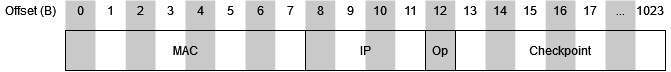
\includegraphics[width=\textwidth]{Images/NAS_message_format.png}
    \caption{Message format expected on the NAS interface.}
    \label{fig:NAS_message_format}
\end{figure}
There are two possible opcodes: An opcode of zero indicates that a checkpoint is being sent to the NAS for it to store, whereas an opcode of one means that a retrieval operation is to be performed. The NAS stores a checkpoint by first instantiating an object with the identifying parameters and the serialised checkpoint sent over Ethernet, now called "snapshot". Because the \verb|<std/vector>| library ported to Genode does not work with non-primitive data types such as the checkpoint object, a doubly linked list is implemented for checkpoint storage. Therefore, a checkpoint has a pointer to both the next and to the previous checkpoint in the list, while the main object of the NAS, in which execution is performed, has a pointer to the last checkpoint of the chain. The last checkpoint was chosen as the one to point to, because checkpoints are added at the end of the list. The class defining such a checkpoint is presented in the following code snippet. 
\newpage
\begin{lstlisting}[language=C++, caption={Checkpoint class used by the NAS.}] 
struct NAS::Checkpoint {
    Genode::uint64_t mac;
    Genode::uint32_t offset;
    Genode::uint8_t *snapshot;

    NAS::Checkpoint *previous;
    NAS::Checkpoint *next;

    Checkpoint(Genode::uint64_t mac, Genode::uint32_t offset, uint8_t *snapshot, NAS::Checkpoint *previous,
               NAS::Checkpoint *next) : mac(mac), offset(offset), snapshot(snapshot), previous(previous), next(next) {}

    ~Checkpoint() = default;
};
\end{lstlisting}
The act of storing a new checkpoint to memory ultimately consists of adding it to the linked list by modifying the necessary fields.
\newline \newline
Checkpoint retrieval is performed by iterating over the linked list by using a \verb|current| checkpoint pointer that, before entering the loop, is set to point to the last checkpoint in the list and at the end of the loop is set to its own predecessor. When the first object of the list, a null pointer, is reached, it is concluded that the checkpoint called for does not exist, upon which an exception is thrown. If the checkpoint could be found, it is sent to the client and removed from the list. The logic described up to this point can be seen in the following listing.
\newpage
\begin{lstlisting}[language=C++, caption={Checkpoint retrieval logic.}] 
auto current = reinterpret_cast<NAS::Checkpoint *>(last);
while (true) {
    if (current == nullptr) {
        Genode::error("Checkpoint for this MAC and offset could not be found");
        break;
    } else if (current->mac == mac && current->offset == offset) {
        Genode::log("Checkpoint retrieved, sending to manager");
        if (send(client, current->snapshot, 1024, 0) != 1024) {
            Genode::error("Message could not be sent");
            shutdown(fd, 0);
            return;
        }

        if (current->previous != nullptr) current->previous->next = current->next;
        if (current->next != nullptr) current->next->previous = current->previous;
        Genode::destroy(sliced_heap, current);
        break;
    }
    current = current->previous;
}
\end{lstlisting}
% !TeX root = ../main.tex
% Add the above to each chapter to make compiling the PDF easier in some editors.

\chapter{Evaluation}\label{chapter:evaluation}
To be regarded as a successful prototype, the following aspects of the CMS need to be operational.
\begin{itemize}
    \item Operational pseudo DSM establishment 
    \item The manager's broker correctly writing the checkpoint to local memory
    \item Successful checkpoint storing within the NAS
    \item Retrieval of the checkpoint of the process for which migration was called
    \item Restoration on the expected RTCR
\end{itemize}
Evaluation was performed by testing the entire process of the RTCR by first establishing a pseudo DSM, sending a checkpoint to the manager and having it store it on the NAS and then calling for migration, which would restore the checkpoint on the other RTCR-dummy running in the system. The checkpoint being sent to the manager in this case is just the name of the RTCR-dummy component it originates from, so that it is possible to trace the two checkpoints to their location of restoration. The initial size of the memory established for DSM purposes is 4096 bytes, with the mentioned checkpoint residing in a eight byte reserved space at an offset of 64 bytes. The values of DSM size and offset were chosen for no specific reason other than to test with non trivial parameters, e.g. an offset of zero. Starting the execution of the system scenario then results in an output of documentation of different breakpoints being reached in the code, and at the end if and what checkpoint reached the migration and restoration interface of the RTCR-dummy. Such an output is presented in the following.
\begin{lstlisting}[caption={Output if no socket connections fail (warnings for invalid signal-context capability omitted).}]
Genode 21.08 <local changes>
232 MiB RAM and 9239 caps assigned to init
[init -> drivers -> nic_drv] --- LAN9118 NIC driver started ---
[init -> drivers -> nic_drv] id/rev:      0x1180001
[init -> drivers -> nic_drv] byte order:  0x87654321
[init -> drivers -> nic_drv] MAC address: 52:54:00:12:34:56
[init -> drivers -> nic_drv] MAC address 52:54:00:12:34:56
[init -> rtcr_dummy_2] lwIP Nic interface down
[init -> nas] lwIP Nic interface down
[init -> manager] lwIP Nic interface down
[init -> nas] lwIP Nic interface up address=10.0.2.2 netmask=0.0.0.0 gateway=0.0.0.0
[init -> manager] lwIP Nic interface up address=10.0.0.2 netmask=0.0.0.0 gateway=0.0.0.0
[init -> rtcr_dummy_2] lwIP Nic interface up address=10.0.1.3 netmask=0.0.0.0 gateway=0.0.0.0
[init -> rtcr_dummy_1] lwIP Nic interface down
[init -> rtcr_dummy_1] lwIP Nic interface up address=10.0.1.2 netmask=0.0.0.0 gateway=0.0.0.0
[init -> manager] Creating root component
[init -> rtcr_dummy_2] Connecting to manager for DSM establishment
[init -> rtcr_dummy_1] Connecting to manager for DSM establishment
[init -> manager] [broker] Connection to broker successful. Establishing DSM on 1025
[init -> manager] [broker] Done updating memory
[init -> manager] [broker] Connection to broker successful. Establishing DSM on 1026
[init -> manager] [broker] Done updating memory
[init -> rtcr_dummy_2] [broker] Notification of new CP sent
[init -> rtcr_dummy_1] [broker] Notification of new CP sent
[init -> manager] [NAS thread] Checkpoint successfully sent to NAS
[init -> nas] Checkpoint was stored successfully
[init -> nas] Checkpoint was stored successfully
[init -> manager] [NAS thread] Checkpoint successfully sent to NAS
[init -> rtcr_dummy_2] Calling for migration
[init -> rtcr_dummy_1] Calling for migration
[init -> nas] Checkpoint retrieved, sending to manager
[init -> nas] Checkpoint retrieved, sending to manager
[init -> rtcr_dummy_1] [Migr thread] Checkpoint dummy_2 received. Migration successful
[init -> rtcr_dummy_2] [Migr thread] Checkpoint dummy_1 received. Migration successful
\end{lstlisting}
Each line of system log is prefaced by the component printing in square brackets, after which follows the name of the thread in additional square brackets. If no thread is specified the main thread of the component is responsible. Lines three to 15 are all automatic prints performed by the lwIP network stack and the NIC-driver and router. Here a first remark has to be made: netmask and gateway are set to all zeroes, even though they were set up differently in the run-script, for reasons unknown. After the network is set up, the manager creates its RPC interface for local access. This interface was not tested, as this would necessitate a completely new system scenario without any networking, because if the manager is set up by the run-script using the network stack, it is not reachable using remote procedure calls. Even if a RTCR-dummy with the same IP as the manager was introduced in the run-script, the two components would not be part of the same machine. Further possibilities to cover this functionality are described in chapter \ref{chapter:limitations_and_future_work}. From line 17 onwards, the main operations are performed. The two dummies set up pseudo DSMs on ports selected by the manager, send a checkpoint which the broker of the manager writes to memory and logs the success thereof. Finally a notification to the manager that a new checkpoint is available is sent. Afterwards the manager spawns respective threads for storing the checkpoints to the NAS. The RTCR-dummies then wait for three seconds before calling for migration, leading to the manager spawning another two threads for retrieving the checkpoints from NAS and selecting a target for each of them, in this case the only available other RTCR-dummy. Successful migration and restoration on the expected RTCRs is then visible by \verb|rtcr_dummy_1| logging the receipt of checkpoint \verb|dummy_2| and vice versa. 
The presented output of the system unfortunately is not always the same. More often than not, one or both of the RTCR-dummy broker print an error indicating that the socket connection to the manager has failed, ultimately resulting in an error thrown by the NAS when both RTCR-dummies call for migration. This happens because one or both RTCRs were never able to send their checkpoints to the manager, which in turn wasn't able to store them to the NAS. The first suspicion was a race condition between the broker and the NIC-router, more specifically, that the broker tries to connect to an uninitialised network stack. This can not be the case, since to be able to spawn a broker, a message has to be successfully received by both the manager and the RTCR. However, as this error only occurs intermittently, a race condition is still suspected.
\newline \newline
Other than that, the main functionalities outlined in the preface of this chapter, operate as conceptualised, resulting in a successful prototype.

% !TeX root = ../main.tex
% Add the above to each chapter to make compiling the PDF easier in some editors.

\chapter{Limitations and Future Work}\label{chapter:limitations_and_future_work}
Even though the fundamental structure of the checkpoint management system is operational as found in chapter \ref{chapter:evaluation}, a few limitations remain which can be improved on. Additionally, this chapter describes possible future work, in which aspects of the CMS and components around it, that where not part of this thesis, could be advanced. 
\subsubsection{Redundancy}
The first limitation is that the conceptualised redundancy of the checkpoint management system was not introduced to the prototypical system scenario. This would necessitate a mutex inside the NAS, so that it is impossible for a checkpoint to be retrieved twice. Furthermore, every time the RTCR-dummies currently contact the manager over network, every redundant manager would have to receive the same information. Therefore the RTCR would also need to know on which IP these are available.
\subsubsection{Distributed Shared Memory}
As already touched on in chapter \ref{chapter:implementation}, the idea of using the DSM implemented by Weidinger, also could not be realised, because porting it to the current version of Genode would have been necessary. Instead of just porting the DSM, it would be more sensible to update the main functionality and integrate that directly into the CMS and RTCR, where instead of using broker components the proposed broker threads are used. 
The current temporary implementation of these brokers also suffers from a race condition: it is possible for the manager to receive the notification by the RTCR that a new checkpoint is available, while the broker has not finished writing it to memory. Fixing this with asynchronous signalling using \verb|Genode::Signal_context| and \verb|Genode::Signal_receiver| was attempted, but eventually postponed. This approach is still regarded as the most likely solution to this issue.
\subsubsection{Dynamic IP and MAC Determination}
Another, albeit small improvement, is to replace the current static, hard-coded IP distribution with a DHCP, and to find a way to determine the values of IP and MAC dynamically inside the code.
\subsubsection{Selection of the Migration Target}
The migration of checkpoints also presents possibilities for improvement. Firstly, the CPU usage of an ECU is currently not part of the metric for migration target selection. If there is a way to determine this value in Genode, this should be incorporated both into the RTCRs system information interface and into the metric itself. The second aspect is that currently the manager refuses migration to the machine that originally called for it. As already mentioned, this needs to be changed so that not only single RTCR system scenarios are possible, but the RTCR is also able to stop execution of the target child when it calls for migration.
\subsubsection{Physical Test Bench and RTCR Integration}
The next step of improving the NAS is to set it up in a real RAID configuration, but since this is only feasible with physical drives, a test bench with multiple ECUs and such a NAS would first have to be configured. Such a physical testing setup would then also allow the proper testing of the RTCR and CMS communication using the RPC interface in case they are on the same ECU. 

Moreover, since the RTCR in the prototypical system scenario is only a dummy, future work also includes integrating the real RTCR into the system. To achieve this, the RTCR has to be ported to the current version of Genode. Furthermore, the necessary interfaces of ECU information and restoration over Ethernet, need to be implemented into the RTCR component. 
\subsubsection{Real-Time Capability}
After such improvements, the CMS has to be tested for real-time capability, preferably using a test bench like the one proposed in the last paragraph. Such a capability is important for the CMS, as the underlying RTCR has it as a requirement, and a manager without it would jeopardise this essential functionality. If these tests imply no real-time capability, concept and implementation of the CMS needs to be improved until this goal is reached.


% !TeX root = ../main.tex
% Add the above to each chapter to make compiling the PDF easier in some editors.

\chapter{Conclusion}\label{chapter:conclusion}
To conclude the thesis, the outcomes of design and implementation are compared to both the research questions asked in \ref{section:research_questions}, and also to each other. Firstly, the main considerations in designing the CMS, after presenting various options, could all be answered in a purposeful discussion leading to a clearly most suitable solution, which was manifested in the final concept of the management system. 
The conceptual question of where in the system such a manager should reside without introducing a single point of failure was answered by a centralised redundant system. This system was designed to receive checkpoints whenever they are created by an RTCR via a hybrid of DSM and publish/subscribe. The secure storage of checkpoints is handled by a NAS component from which checkpoints can be retrieved for migration and restoration. Available RAM, available capabilities and CPU status where selected as metrics to distinguish ECUs from another for migration suitability, answering the final research question.

Unfortunately, some aspects of these concepts could not be fully implemented. This includes the introduction of the CMS as a single point of failure, as a redundant manager was not introduced and tested. Also, the realisation of Weidinger's distributed shared memory, the completely secure storage of checkpoints because of missing RAID configuration of the NAS, and the inclusion of an ECUs CPU usage in the metrics for selecting a migration target are absent. However, a basis for further work with operational main functionalities of sending, storing, retrieving, migrating, and restoring checkpoints could be established, resulting in a successful proof of concept. 

Overall, it seems that the concept could address the problem of checkpoint management in the right way, and after correcting the limitations it could be usefully integrated into the vision of KIA4SM.

\appendix{}

\microtypesetup{protrusion=false}
\listoffigures{}
%\listoftables{}
\lstlistoflistings
\microtypesetup{protrusion=true}
\printbibliography{}

\end{document}
